\section{Zielsetzung}
Das Ziel des vorliegenden Versuches ist es, das Energiespektrum des Krebsnebels aus rekonstruierten Gamma-Ereignissen, welche durch das FACT-Experiment aufgenommen wurden, zu bestimmen. Dazu wird mit Hilfe von Entfaltungsmethoden aus den geschätzten Energien und den Detektoreigenschaften das ursprünglich emittierte Spektrum bestimmt.

\section{Theorie}
Ein bedeutender Teil der Astroteilchenphysik ist der Nachweis und die Interpretation von astronomischen Botenteilchen. Anhand verschiedener Merkmale lassen sich Rückschlüsse auf die Quelle der Botenteilchen und somit auf Strukturen und Ereignisse im Universum ziehen. Die Botenteilchen lassen sich in drei Kategorien einteilen: Die geladene kosmische Strahlung, Neutrinos und Photonen. 
Abbildung \ref{fig:Boten} zeigt schematisch die drei Arten von Botenteilchen und ihren Weg von der Quelle zur Erde.
\begin{figure}
  \centering
  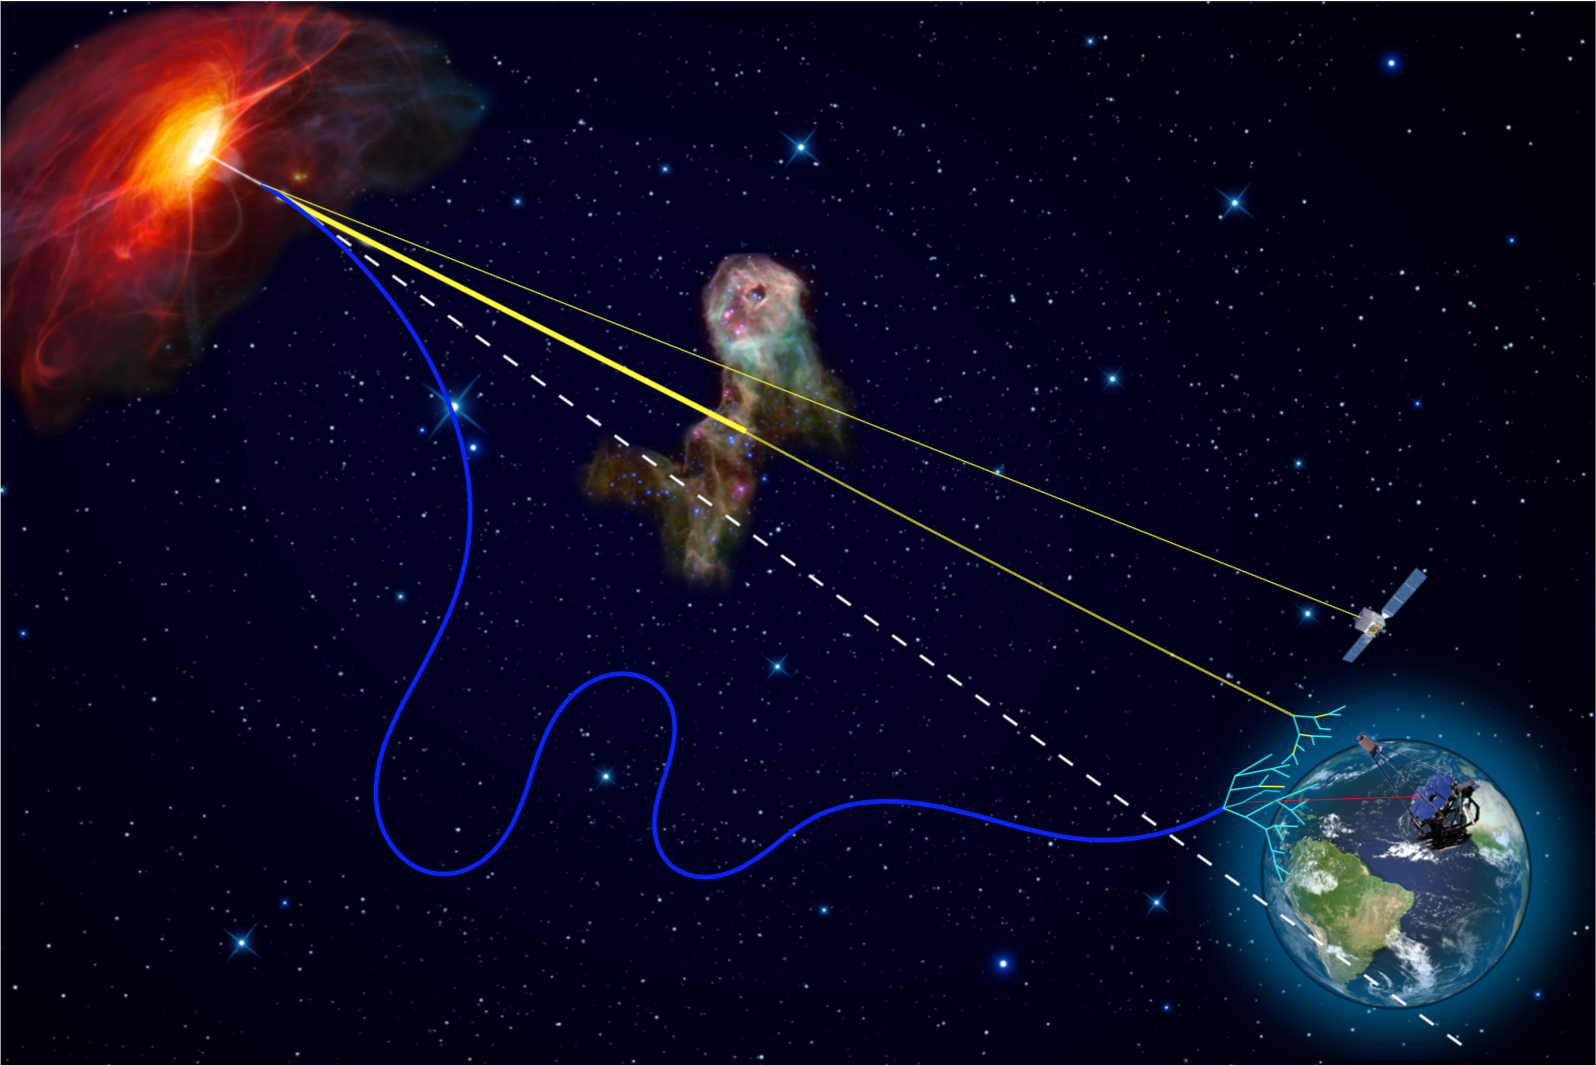
\includegraphics[width=0.6\textwidth]{graphics/Folie5.png}
  \caption{Schematische Darstellung von astrophysikalischen Botenteilchen auf ihrem Weg von der Quelle zur Erde. Die blaue Linie stellt geladene Teilchen dar, die Neutrinos werden durch die gestrichelte Linie veranschaulicht und die Photonen durch die Gelbe.\cite{anleitung}}
  \label{fig:Boten}
\end{figure}
\FloatBarrier
Tscherenkow-Teleskope, wie das FACT-Teleskop, machen sich die Wechselwirkungen von hochenergetischen Photonen mit der Atmosphäre zunutze. Hierbei entstehen Teilchenkaskaden, welche sich zum Teil schneller als die Lichtgeschwindigkeit des durchquerten Mediums bewegen und somit Tscherenkow-Licht in Form eines Kegels emittieren. Dieses wird von den Teleskopen aufgenommen und ausgewertet.
Da die Photonen ungeladen sind, erfahren sie auf ihrem Weg zur Erde keine Ablenkung durch Magnetfelder. Dadurch bleiben die Richtungsinformationen erhalten und können zur Bestimmung der Quelle verwendet werden.
Die Teilchenkaskaden werden jedoch nicht nur durch Photonen, sondern ebenfalls durch geladene Botenteilchen wie zum Beispiel Protonen verursacht. Da diese in der Gammaastronomie als Hintergrund zählen, müssen diese Ereignisse von den Gamma-Ereignissen getrennt werden.


%In der Astroteilchenphysik werden die sogenannten Botenteilchen, die von Quellen ausgesendet werden, in drei Kategorien eingeteilt. Die geladene kosmische Strahlung wird durch Magnetfelder im intergalaktischen und interstellarem Medium abgelenkt. Deshalb lässt sich zwar bedingt auf ihre Ladung zurückschließen, aber die Richtungsinformation zu ihrer Quelle geht verloren. Eine weitere Kategorie bilden die Neutrinos. Sie sind durch ihren extrem kleinen Wirkungsquerschnitt nur schwer nachzuweisen. Durch ihre neutrale Ladung werden sie jedoch nicht abgelenkt und besitzen somit grundsätzlich eine Richtungsinformation. Die aktuelle Forschung beschäftigt sich mit den ersten Hinweisen zu Neutrinopunktquellen. Die dritte Kategorie bilden die hochenergetischen Photonen. Sie übermitteln die Richtungsinformation zu ihrer Quelle und können sowohl direkt mit Satelliten nachgewiesen werden oder mit bodengebundenen Tscherenkow-Teleskopen.

%Diese machen sich die Wechselwirkungen von hochenergetischen Photonen mit der Atmosphäre zunutze, wobei Teilchenkaskaden erzeugt werden. Diese bewegen sich zum Teil im Medium überlichtschnell, sodass es zur Abstrahlung von Tscherenkowlicht kommt. Dieses wird von den Teleskopen gemessen. Die Teilchenkaskaden werden jedoch nicht nur durch Photonen, sondern ebenfalls durch geladene Botenteilchen wie zum Beispiel Protonen verursacht. Die Abbildung \ref{fig:Boten} zeigt schematisch die drei Arten von Botenteilchen und ihren Weg von der Quelle zur Erde.\\
%\begin{figure}
%  \centering
%  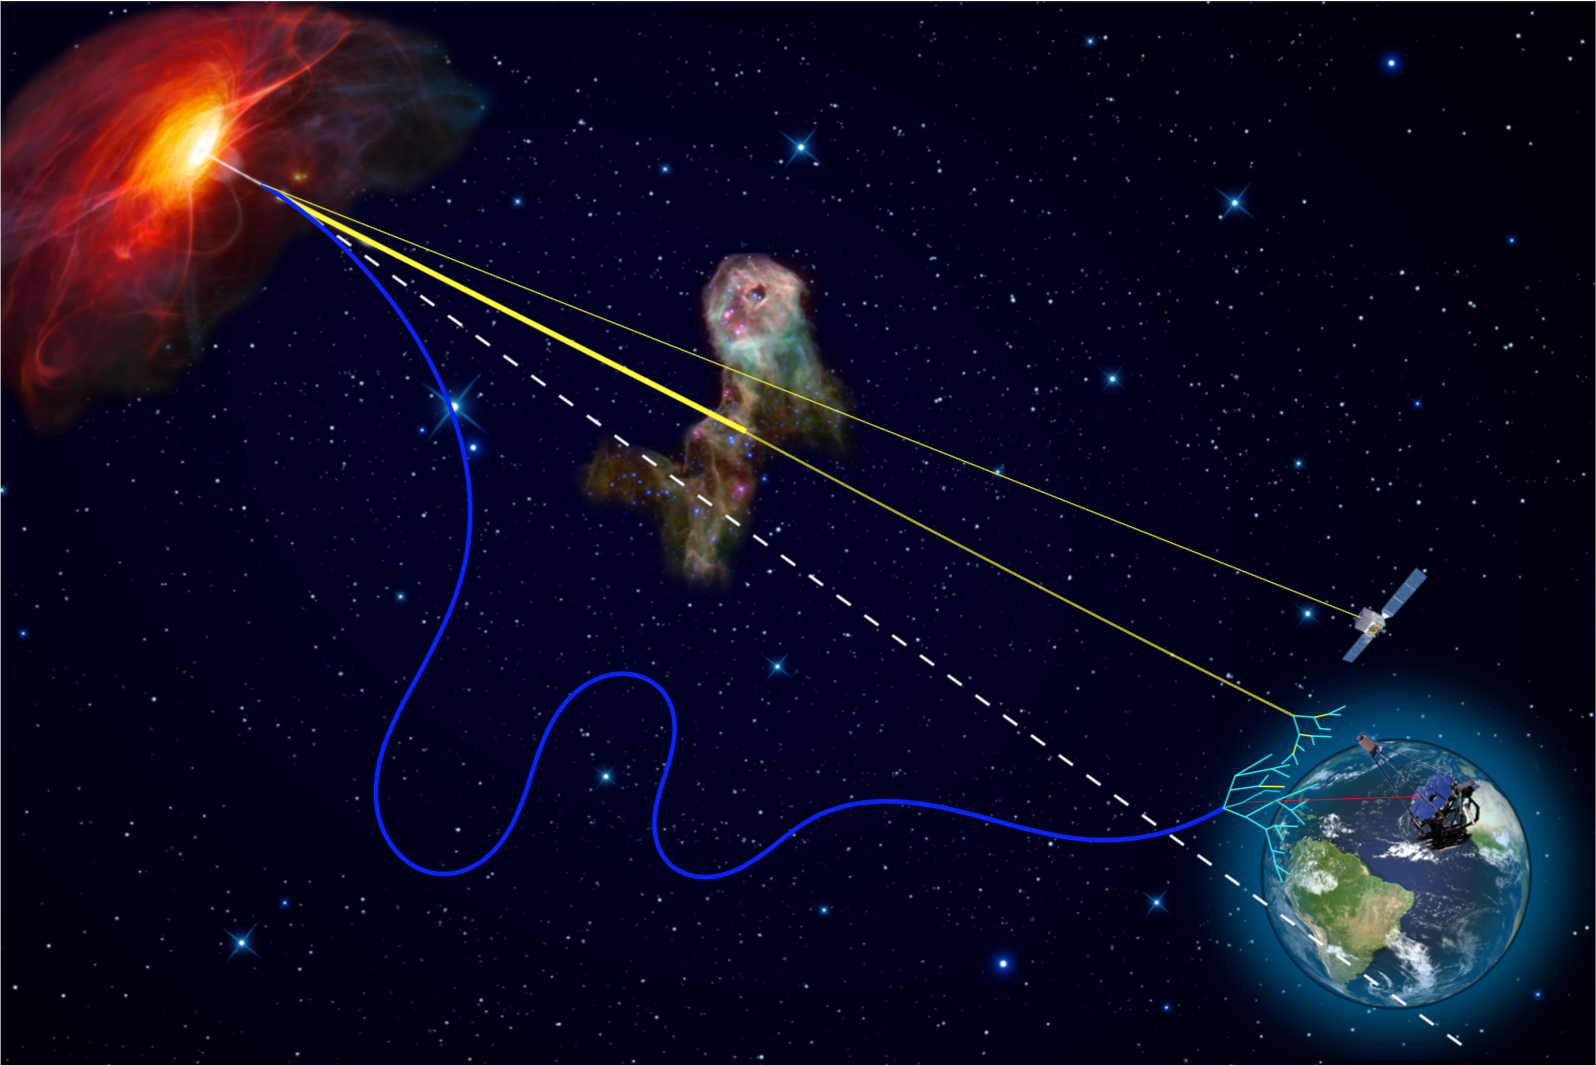
\includegraphics[width=0.6\textwidth]{graphics/Folie5.png}
%  \caption{Schematische Darstellung von astrophysikalischen Botenteilchen auf ihrem Weg von %der Quelle zur Erde. Die blaue Linie stellt geladene Teilchen dar, die Neutrinos werden %durch die gestrichelte Linie veranschaulicht und die Photonen durch die Gelbe.\cite%{anleitung}}
%  \label{fig:Boten}
%\end{figure}
%Der vorliegende Versuch beschäftigt sich mit der Gammaastronomie und somit den Photonen als Botenteilchen.
\subsection{FACT}
Das \textit{First G-APD Cherenkov Telescope}, \cite{Anderhub_2013} kurz FACT, ist ein bodengebundenes, abbildendes Tscherenkow-Teleskop, welches in Abbildung \ref{fig:FACT} zu erkennen ist. Seit 2011 operiert es im  im Obersatorio del Roque de los Muchachos auf La Palma, wo es aufgrund der geringen Lichtverschmutzung platziert wurde.
Beobachtet werden Quellen von hochenergetischen Photonen, wie zum Beispiel dem Supernovaüberrest Krebsnebel. Des Weiteren dient das FACT-Teleskop zum Testen der Anwendung von siliziumbasierten Halbleiterphotodetektoren, den sogenannten G-APD, in der Gammaastronomie. Diese bieten eine höhere Robustheit und haben eine größere Detektionseffizienz, sodass eine höhere Sensitivität der Kamera vermutet wird. \cite{FACTside, Anderhub_2013} 
\begin{figure}
  \centering
  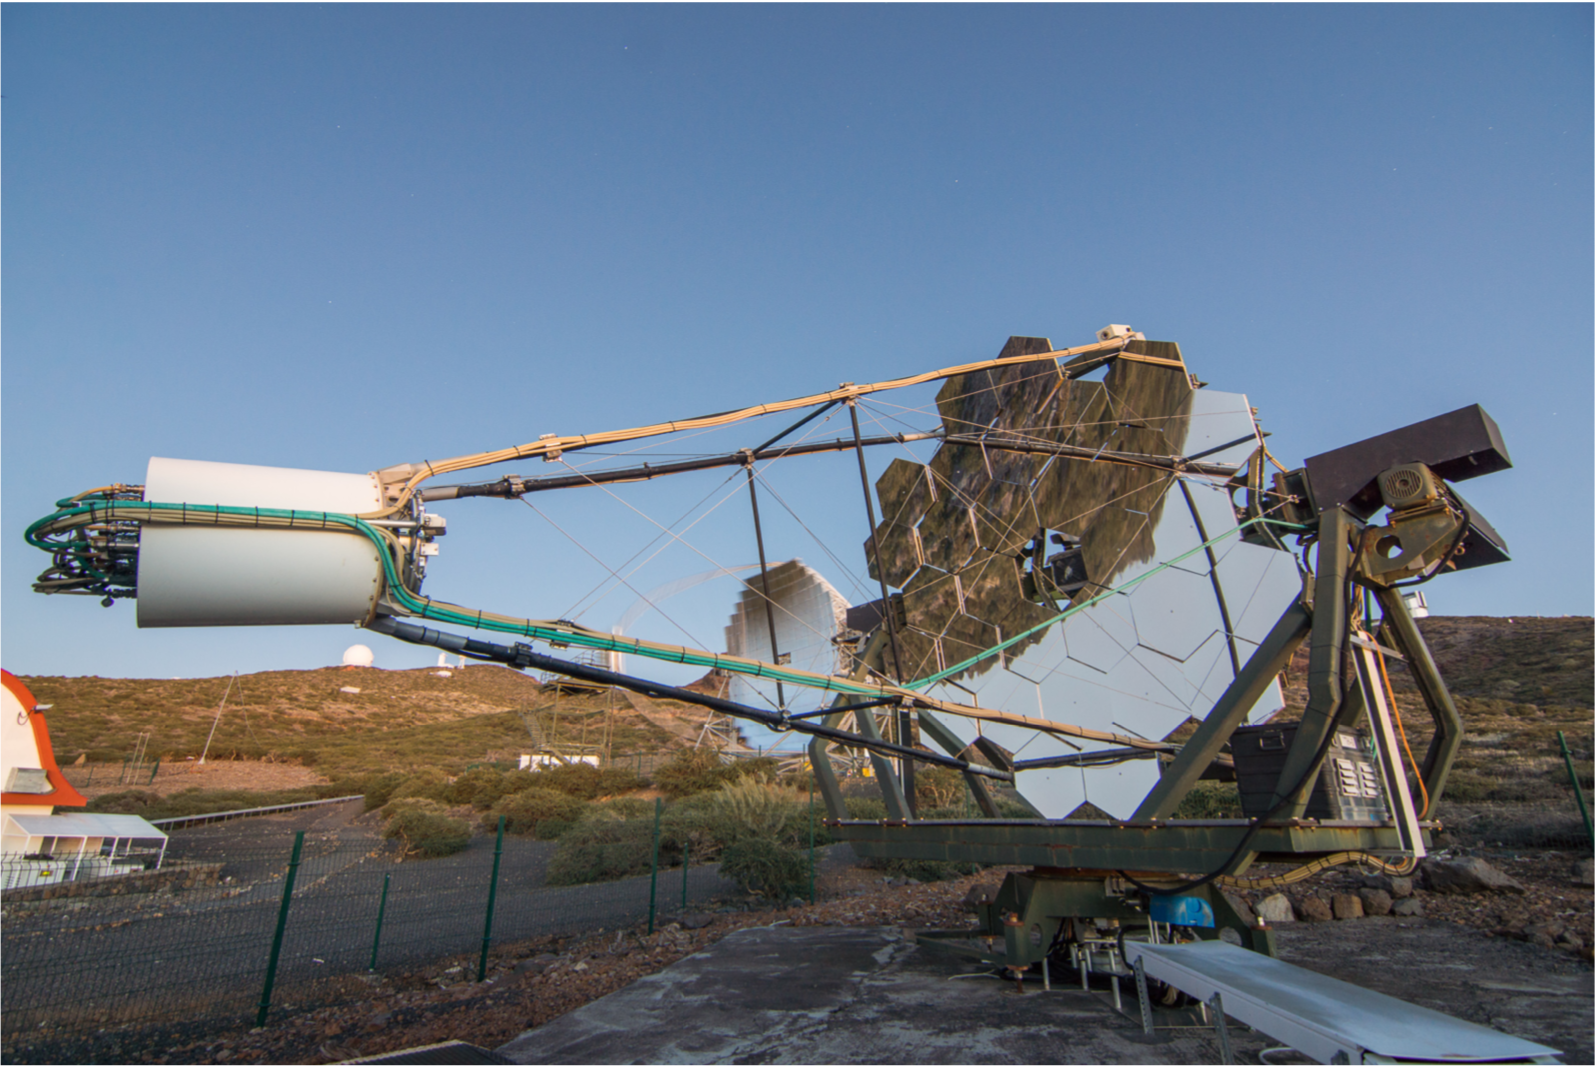
\includegraphics[width=0.8\textwidth]{graphics/Max.png}
  \caption{ Fotografie des FACT-Teleskopes. In dem weißen Zylinder befindet sich die Kamera, welche aus den G-APDs besteht. [M. Nöthe, 2018]}
  \label{fig:FACT}
\end{figure}


\subsection{Entfaltung}
Teleskope sind nicht in der Lage, alle physikalische Größen direkt zu messen. So werden in der Astrophysik in der Regel Ladungsdepositionen der Teilchen im Detektormaterial aufgenommen, aus welchen im Anschluss die Eigenschaften des Primärteilchen rekonstruiert werden. Auch das Detektionsverfahren hat, zum Beispiel in Form von Detektionseffizienzen,  einen Einfluss auf die Messwerte.
Die Verteilung $g(y)$ der gemessenen Größe $y$ kann mit der Fredholmschen-Integralgleichung erster Art
\begin{align}
	g(y)=\int A(y,x)f(x)\text{d}x + b(y)
	\label{eqn:1}
\end{align}
ausgedrückt werden. Die Verteilung der physikalischen Größe $x$ wird dabei durch $f(x)$ beschrieben, während der Untergrund durch $b(y)$ und der Faltungskern durch $A(y,x)$ dargestellt ist. Unter dem Letzteren sind die Eigenschaften des Detektors zusammengefasst. Dieser wird aus Simulationsdaten ermittelt, während der Untergrund aus den Off-Messungen bestimmt werden kann.

Um aus der gemessenen Verteilung $g(y)$ die physikalische Verteilung $f(x)$ zu erhalten, können Entfaltungsmethoden angewendet werden.
Hierzu werden die Verteilungen zunächst durch Histogramme dargestellt, wodurch die Verteilungen aus Gleichung \eqref{eqn:1} zu Vektoren und der Faltungskern zu einer Matrix transformiert werden. Die Fredholmsche-Integralgleichung erster Art kann somit als 
\begin{align}
	\vec{\pmb{g}} = \pmb{A}\vec{\pmb{f}} + \vec{\pmb{b}}
	\label{eqn:2}
\end{align}
dargestellt werden.
Um einen Schätzer für die physikalische Größe zu erhalten, muss \eqref{eqn:2} invertiert werden. 

%Der $M$-dimensionale Vektor $\vec{\pmb{g}}$ steht für das Histogramm der geschätzten Gamma-Energien für alle gemessenen Photonen. Der ebenfalls $M$-dimensionale Vektor $\vec{\pmb{b}}$ beschreibt das Untergrundhistogramm und lässt sich aus den Off-Messungen ableiten. Der $N$-dimensionale Vektor $\vec{\pmb{f}}$ beschreibt die wahren Gamma-Energien und die $M\times N$-dimensionale Matrix $\pmb{A}$ stellt die Migrationsmatrix des Energieschätzers dar. \\
%Von diesem Punkt aus kann nun der Schätzer $\hat{\vec{f}}$ bestimmt werden. Die Akzeptanzkorrektur kann entweder zuletzt auf den Schätzer $\hat{\vec{f}}$ angewendet werden oder die Migrationsmatrix $\pmb{A}$ muss zu Beginn geeignet normiert werden.

\subsubsection{Naive SVD-Entfaltung}
Die Naive SVD-Entfaltung bildet die einfachste, aber auch fehleranfälligste Möglichkeit einer Entfaltung. 
Hierzu wird die Migrationsmatrix des Energieschätzers $\pmb{A}$ invertriert, indem die Moore-Penrose-Pseudoinverse berechnet wird. Der Schätzer für die physikalische Größe kann anschließend über
\begin{align}
	\hat{\vec{\pmb{f}}} = \pmb{A}^{+}(\vec{\pmb{g}} - \vec{\pmb{b}})
	\label{eqn:NSVD}
\end{align}
ermittelt werden.

\subsubsection{Poisson-Likelihood-Enfaltung}
Als zweite Möglichkeit kann eine Likelihood-Entfaltung angewendet werden. 
Hierfür wird die Annahme getroffen, dass die Messgröße poissonverteilt ist und somit der Wahrscheinlichkeitsverteilung
\begin{align}
	P(g_{i}) &= \mathcal{P}(g_{i},\lambda_{i}) \; \text{mit}\\
	\vec{\pmb{\lambda}} &= \pmb{A} \cdot \vec{\pmb{f}} + \vec{\pmb{b}}
\end{align}
folgt.
Die Likelihood der Poissonverteilung ergibt sich zu
\begin{align}
	\mathcal{L} = \prod_{i=1}^{M}\mathcal{P}(g_{i},\lambda_{i})
\end{align}
Numerisch ist es jedoch sinnvoller die negative Log-Likelihood zu minimieren
\begin{align}
	- \ln\mathcal{L} = - \sum_{i=1}^{M}\mathcal{P}(g_{i},\lambda_{i}) = \sum_{i=1}^{M}\ln(g_{i}!) - g_{i} \cdot \ln \lambda_{i} +\lambda_{i}
	\label{eqn:loglike}
\end{align}
sodass sich der Schätzer $\vec{\pmb{f}}$ zu:
\begin{align}
	\hat{\vec{\pmb{f}}} = \text{argmin}\left(- \ln\mathcal{L}( \vec{\pmb{f}}|\pmb{A},\vec{\pmb{g}},\vec{\pmb{b}})\right)
	\label{eqn:fLike}
\end{align}
ergibt.

\section{Datensatz}
Für den durchzuführenden Versuch liegt ein aufbereiteter Datensatz bzw. mehrere im Datenlevel 3 vor, welche im folgenden aufgeführt sind.
\begin{itemize}
	\item \textit{open\_crab\_sample\_dl3.hdf5} Messdaten aus \SI{17.7}{\hour} Oberservationszeit des Krebsnebels.
	\item \textit{gamma\_test\_dl3.hdf5} Testdatensatz bestehend aus \SI{70}{\percent} der ursprünglichen simulierten Quell-Gammas.
	\item \textit{gamma\_corsika\_v1.1.2.hdf5} Informationen über alle simulierten Gamma-Luftschauer.
\end{itemize}
Aus den Messdaten des FACT-Teleskops wurden die Eigenschaften \textbf{Teilchenklasse, Energie} und \textbf{Herkunftsrichtung} der Primärteilchen rekonstruiert.
Um dies zu ermöglichen werden die Daten zunächst mit den \textbf{FACT-Tools} \cite{kai_brugge_2018_2386762} analysiert. 
%Dabei wird zunächst die Spannungszeitreihe von jedem Pixel kalibriert und anschließend die Anzahl der Photonen und deren mittlere Ankunftszeit in jedem Pixel ermittelt. Aus diesen werden nun die Pixel ausgewählt, die ein Tscherenkow-Signal enthalten. Zuletzt erfolgt die Parametrisierung des Schauerbildes mit Hilfe der Hillas-Parameter. Diese sind in Abbildung \ref{fig:Para} dargestellt.
%\begin{figure}
%	\centering
%	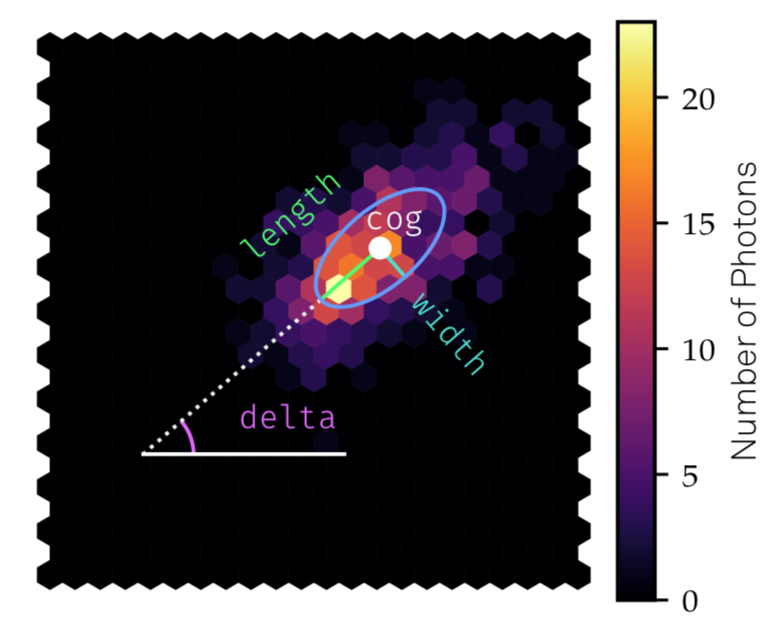
\includegraphics[width=0.6\textwidth]{graphics/Hillas.png}
%	\caption{Schauerbild eines Photons mit  den wichtigstens Hillas-Parametern. Der %Mittelpunkt wird als \textit{cog} bezeichnet, die beiden Standardabweichungen \textit%{length} und \textit{width} stammen aus der Hauptkomponentenanalyse der %2d-Lichtverteilung. Die Orientierung der Hauptachse des Schauers wird mit dem Winkel %\textit{delta} zur x-Achse angegeben.\cite{anleitung}}
%	\label{fig:Para}
%\end{figure}
%Anschließend werden Methoden des Maschinellen Lernens verwendet, um die Teilcheneigenschaften zu bestimmen. Dazu werden zunächst Simulationen für einen Testdatensatz durchgeführt, aus diesem lässt sich ebenfalls die Detektorakzeptanz bestimmen. \\
%Mit dem Programm \textbf{CORSIKA} \cite{1998cmcc.book.....H} lässt sich die Produktion der Luftschauer und das anschließend entstehende Tscherenkowlicht, das den Detektor erreicht, simulieren. Dafür werden als Eingabewerte die Eigenschaften des Primärteilchens genutzt. Mit dem Programm \textbf{CERES} lässt sich anschließend das FACT-Teleskop simulieren. Dabei werden nicht nur Eigenschaften wie die Spiegel und Kamera-Elektronik beachtet, sondern die Daten am Ende im selben Datenformat wie die eigentlichen Messdaten gespeichert. Der entscheidende Unterschied ist, dass die Informationen über das Primärteilchen erhalten sind.\\
%Um zusätzlich den Untergrund abschätzen zu können, werden drei Datensätze simuliert.
%\begin{itemize}
%	\item Gammas, aus einer punktförmigen Quelle, die im Wobble-Modus beobachtet wird
%	\item Gammas, die diffus aus zufälligen Orten ins Blickfeld des Teleskop kommen
%	\item Protonen, die diffus aus zufälligen Orten ins Blickfeld des Teleskop kommen
%\end{itemize}
%Die Teilchenart wird mithilfe eines Random Forest Klassifikator bestimmt, dieser wurde darauf trainiert, diffuse Gammas von den Protonen zu unterscheiden. Der Energieschätzer ist ein Random Forest Regressor, der die Quellgammas als Trainingsdaten nutzt. Die Richtungsrekonstruktion wurde mithilfe der \textit{disp}-Methode durchgeführt. Die eigentliche 2d-Regression für den Herkunftsort der Teilchen reduziert sich dabei auf eine 1-Dimensionale unter der Annahme, dass die Quelle auf der Hauptachse vom Schwerpunkt des Schauers liegt. Zudem erhält man eine binäre Klassifikation in welche der beiden möglichen Richtungen auf der Hauptache die Quelle liegt.\\
%Aus dieser Analyse entstehen die oben aufgeführten Datensätze, die unter \cite{FACTdata} heruntergeladen werden können.
Hiermit werden jene Pixel ausgewählt, welche ein Tscherenkow-Signal enthalten und die Teilchenschauer parametrisiert. Die Abschätzung der Teilcheneigenschaften erfolgt durch Methoden des Maschinellen Lernens. Hierzu werden Simulationen der Teilchenschauer, sowie des Teleskopes zur Hilfe genommen. Der Lerner ist anschließend in der Lage, das Primärteilchen zu klassifizieren, dessen Energie sowie die grobe Herkunftsrichtung abzuschätzen.
Neben den Messdaten des FACT-Teleskopes stehen auch die simulierten Daten, wie oben aufgeführt, zur Verfügung.